\newpage
\section{Descrição dos dados e fontes}
\label{sec:descricao}

\begin{table}[htb]
\IBGEtab{\caption{Estatística descritiva e fonte das principais variáveis}
\label{table:tabela3}
}{%
\bgroup
\def\arraystretch{1.5}
\begin{tabular}{p{3cm}p{8.5cm}cc}
\toprule
\textbf{Variável} & \textbf{Fontes} & \textbf{Média} & \textbf{Desvio-Padrão} \\
\midrule
Coalizões sobredimensionadas & Compilada pelo autor a partir de dados sobre a composição partidária dos gabinetes presidenciais cedidos por Octavio Amorim Neto e Cecília Martinez-Gallardo, relatórios mensais do \textit{CIA World Leaders} e \textit{Lexis Nexis Academics}. Adicionalmente, os dados foram checados com os de Cheibub (\citeyear{cheibub2007}), Chasquetti (\citeyear{chasquetti2001}) e Saez e Montero (\citeyear{alcantara2008}) e confirmados por especialistas. O número de cadeiras no congresso (câmara baixa, no caso de países bicamerais) foram extraídos de Nohlen (\citeyear{nohlen2005}), \textit{Political Database of the Americas} e \textit{Observatório del Poder Legislativo en América Latina}. & 0.17 & 0.37 \\
Número de partidos extras & Compilada pelo autor a partir das fontes descritas acima. & 0.34 & 0.99 \\
Índice de poder presidencial (Negretto) & Extraída de Negretto (\citeyear{negretto2013}). Varia de 0 a 100. & 53.39 & 24.53 \\
Poder presidencial de veto & Extraída de Negretto (\citeyear{negretto2013}). Estandardizada para ficar entre 0 e 1. & 0.58 & 0.19 \\
Controle do orçamento & Extraída de Cheibub (\citeyear{cheibub2007}). \textit{Dummy}. & 0.76 & 0.42 \\
Polcon 3 & Extraída de Henisz (\citeyear{henisz2002}). Varia de 0 a 1.  & 0.36 & 0.14 \\
Efetividade do legislativo & Extraída do \textit{Global Competitiveness Report} do \textit{World Economic Forum} e compilada por Stein et al. (\citeyear{stein2006}). Varia entre 0 e 7.  & 2.22 & 0.58 \\
Extremismo do presidentes & Compilada pelo autor a partir de um banco de dados contendo todos os partidos políticos com mais de 5\% de cadeiras no congresso nos 18 países da América Latina, aos quais foram atribuídos \textit{scores} de 0, mais à esquerda, a 5, mais a direita, extraídos de três classificações diferentes: a de Coppedge (\citeyear{coppedge1997}), ampliada por Baker e Greene (\citeyear{baker2011}), a de Alcántara (\citeyear{alcantara2012}) e a de Wiesehomeier e Benoit (\citeyear{wie2009}) -- estas últimas estandardizadas para tornarem-se compatíveis com a classificação descreta. A variável usada no artigo privilegia a classificação de Alcántara e preenche os \textit{missings} com, respectivamente, os dados de Wiesehomeier e Benoit, de Coppedge e de Baker e Greene.       & 0.9 & 0.9 \\
Polarização no congresso & Compilada pelo autor a partir das fontes descritas acima. & 0.3 & 0.18 \\
Ciclo eleitoral & Compilada pelo autor a partir do \textit{Political Database of the Americas}. Varia entre 0 e 1. & 0.54 & 0.35 \\
Taxa anual média de inflação & Extraída do \textit{World Development Indicators}. Foi \textit{standardizada} para ter a mínima 0 e transformada em logaritmo. & 3.69 & 1.25 \\

\bottomrule
\end{tabular}
\egroup
%
}{ }
\end{table}
\newpage

\section{Testes de Robustez}
\label{sec:robustez}

Nos modelos 6, 7, 8 e 9 da~\hyperref[table:tabela2]{Tabela 2}, apenas os seis países com ocorrência de coalizões sobredimensionadas no período foram analisados, gerando, assim, uma amostra mais balanceada\footnote{Em nenhum deles a variável \textit{Efetividade do Legislativo}, já que, por ter observações incompletas, a sua inclusão reduziria ainda mais o tamanho da amostra.}. Embora os resultados não se alterem substancialmente, o descarte das demais observações implica que esta amostra não é minimamente representativa da América Latina e, por isso, os resultados não podem ser generalizados. 

\begin{table}[htp]
\IBGEtab{\caption{Determinantes da ocorrência de coalizões governamentais sobredimensionadas em seis países da América Latina, 1979-2012}
\label{table:tabela4}
}{%
\begin{tabular}{lcccc}
\toprule
{} & \textbf{Modelo 6} & \textbf{Modelo 7} & \textbf{Modelo 8} & \textbf{Modelo 9} \\
\midrule
Número efetivo de partidos & 0.38* & 0.20 & 0.35*** & 0.29*** \\
{} & (0.21) & (0.23) & (0.09) & (0.07) \\
Força do legislativo (Polcon3) & 5.98*** & 6.5*** & 1.65* & 1.7** \\
{} & (1.83) & (1.75) & (0.88) & (0.79) \\
Poder presidencial (Negretto) & 0.05** & & 0.02** &  \\
{} & (0.02) & & (0.01) &  \\
Poder de veto & & -7.69 & & -2.29 \\
{} & & (4.97) &  & (1.68) \\
Controle do orçamento & & 1.84 &  & 0.58 \\
{} & & (1.24) &  & (0.72) \\
Decreto legislativo & & -0.41 &  & -0.11 \\
{} & & (2.12) &  & (0.64) \\
\% de cadeiras do presidente & 9.88*** & 9.69*** & 3.66**  & 3.54*** \\
{} & (3.12) & (2.82) & (1.58) & (1.34) \\
Extremismo do presidente & -1.74*** & -1.59*** & -0.65** & -0.72*** \\
{} & (0.54) & (0.43) & (0.27)  & (0.16) \\
Polarização no congresso & -3.42 & 0.37 & -0.22 & 1.07 \\
{} & (4.14) & (5.12) & (2.46) & (2.28) \\
Ciclo eleitoral & 1.08** & 1.19** & 0.47 & 0.54* \\
{} & (0.55) & (0.55) & (0.37) & (0.31) \\
Inflação_{log} & -0.48** & -0.64* & -0.26** & -0.31*** \\
{} & (0.23) & (0.34) & (0.1) & (0.09) \\
Log-likelihood & -67.7 & -66.15 & -159.46 & -158.18 \\
Clusters & 36 & 36 & 36 & 36 \\
N & 154 & 154 & 154 & 154 \\
\bottomrule
\end{tabular}%
}{%
\nota{$\ast\ast\ast p<0.01; \ast\ast p<0.05; \ast p< 0.1$. Os modelos foram estimados por \textit{maximum likelihood}. Erros-padrão robustos com \textit{cluster} para os presidentes entre parênteses. As constantes foram omitidas e a variável inflação foi atrasada.}
}
\end{table}

Como os resultados indicam, não existem alterações na significância e no sinal das principais variáveis, embora algumas modificações sejam perceptíveis. Nos modelos 6 e 7, que inclui efeitos-fixos para os países e o indicador binário de presença de coalizões \textit{surplus} como variável dependente, o efeito da polarização ideológica apresenta sinais opostos, mas acompanhas de erros grandes. Apesar do pequeno número de casos, o Número Efetivo de Partidos Parlamentares, o poder do presidente e força do congresso atingem níveis de significância. Todo resto fixado na média, a diferença na probabilidade de formar uma coalizão sobredimensionada entre o presidente com maior \textit{score} no índice de poder presidencial e o menor é de 29\%; entre o congresso mais forte e o mais fraco, de 13\%; e, entre um congresso com 2 e 10 partidos efetivos, 5\%. À exceção da fragmentação partidária, portanto, o impacto dos poderes legislativos do presidente e da capacidade do congresso de impedir mudanças no \textit{status quo} se mantêm nesta amostra reduzida.
 
Nos modelos 8 e 9, por fim, o número de partidos adicionais foi novamente utilizado como variável dependente. De forma semelhante aos modelos 4 e 5, os sinais das variáveis de interesse se mantêm e quase todas atingem níveis convencionais de significância -- à exceção, também aqui, dos três indicadores de poderes presidenciais no modelo 9. Controlando os demais preditores neste, o congresso mais forte da amostra gera um número esperado de partidos adicionais de 0.29, contra 0 de outro com a menor força registrada. No caso do poder presidencial, segundo a estimativa do modelo 4, esse valor vai de 0.24 a 0.02 partidos adicionais, para o presidente mais forte e mais fraco na amostra, respectivamente. Ao contrário, polarização, extremismo do presidente e Número Efetivo de Partidos apresentam todos impacto reduzido em ambos os modelos.

\begin{table}[!htbp]
\IBGEtab{\caption{Determinantes da ocorrência de coalizões governamentais sobredimensionadas na América Latina, 1979-2012 (posições ideológicas compiladas a partir de outras fontes)}
\label{table:tabela5}
}{%
\begin{tabular}{lcccc}
\toprule
{} & \textbf{A} & \textbf{B} & \textbf{C} & \textbf{D} \\
\midrule
Número efetivo de partidos & 0.25* & 0.53** & 0.24* & 0.52**  \\
{} & (0.13) & (0.25) & (0.14) & (0.22)   \\
Força do legislativo (Polcon3) & 2.7 & 4.34* & 3.09* & 6.57**   \\
{} & (1.89) & (2.67) & (1.79) & (2.98)   \\
Poder presidencial & 0.04*** & 0.05* & 0.02 & 0.00   \\
{} & (0.01) & (0.03) & (0.01) & (0.03)  \\
Efetividade do legislativo & & 0.21 & & 1.35   \\
{} & & (1.11) & & (1.4)   \\
Extremismo do presidente (Baker e Greene) & -0.99** & -0.89 &  &   \\
{} & (0.51) & (0.67) &  &    \\
Polarização no congresso (Baker e Greene) & -5.95** & -9.83** &  &   \\
{} & (2.88) & (4.96) &  &    \\
Extremismo do presidente (Coppedge) & & & -0.39** & -0.2***   \\
{} &  &  & (0.33) & (0.59)   \\
Polarização no congresso (Coppedge) & & & -10.61*** & -21.76**   \\
{} & & & (3.71) & (9.29)  \\
Ciclo eleitoral & 1.71** & 2.63** & 1.52* & 2.46*  \\
{} & (0.88) & (1.11) & (0.85) & (1.19)  \\
\% de cadeiras do presidente & 8.01*** & 12.05*** & 7.73*** & 12.4***  \\
{} & (2.62) & (2.93) & (2.51) & (3.2)  \\
Inflação_{log} & -0.45* & -0.60** & -0.33 & -0.58  \\
{} & (0.25) & (0.37) & (0.22) & (0.41)  \\
$t$ & -4.73*** & -4.85*** & -4.37*** & -3.96***   \\
{} & (0.85) & (1.33) & (0.8) & (1.18)   \\
$t^{2}$ & 0.74*** & 0.76*** & 0.67** & 0.57***   \\
{} & (0.15) & (0.24) & (0.15)& (0.2)  \\
$t^{3}$ & -0.03*** & -0.03*** & -0.03** & -0.02***  \\
{} & (0.01) & (0.01) & (0.1) & (0.00)  \\
Log-likelihood & -56.42 & -31.81 & -55.16 & -28.48  \\
Clusters & 102 & 82 & 102 & 82   \\
N & 421 & 328 & 421 & 421   \\
\bottomrule
\end{tabular}%
}{ %
\nota{$\ast\ast\ast p<0.01; \ast\ast p<0.05; \ast p< 0.1$. Os modelos foram estimados por \textit{maximum likelihood}. Erros-padrão robustos com \textit{cluster} para os presidentes entre parênteses. As constantes foram omitidas e a variável inflação foi atrasada. Nos modelos A e B, as posições ideológicas dos partidos latino-americanos foram compiladas a partir dos dados de Baker e Greene (\citeyear{baker2011}), mas a variável final foi estandardizada e centrada. Nos modelos C e D, a posição dos partidos foi extraída de Coppdge (\citeyear{coppedge1997}), atualizadas por Baker e Greene (\citeyear{baker2011}).}
}
\end{table}


\begin{table}[!htbp]
\IBGEtab{\caption{Determinantes da ocorrência de coalizões governamentais sobredimensionadas na América Latina, 1979-2012 (controles adicionais)}
\label{table:tabela6}
}{%
\begin{tabular}{lccccc}
\toprule
{} & \textbf{E} & \textbf{F} & \textbf{G} & \textbf{H} & \textbf{I} \\
\midrule
Número efetivo de partidos & 0.39  & 0.22 & 0.06 & 0.16 & 0.08  \\
{} & (0.29)  & (0.15) & (0.17) & (0.17) & (0.18)  \\
Força do legislativo (Polcon3) & 6.22*** & 4.39** & 0.58** & 4.82*** & 5.21***  \\
{} & (2.37) & (1.74) & (1.68) & (1.77) & (1.68)  \\
Poder presidencial (Prespow2) & -3.61 & 0.65 & 5.02 & &  \\
{} & (3.9) & (2.31) & (3.38) &  &  \\
Poder presidencial (Negretto) & & & & 0.02 & 0.02 \\
{} & & & & (0.02) & (0.02)  \\
Efetividade do legislativo & 2.20** & & & &  \\
{} & (1.15) & & & &   \\
Controle da lista partidária & & 1.33** & 1.54** & 1.02* & 1.43** \\
{} & & (0.63) & (0.71) & (0.58) & (0.61)  \\
Status Freedom House &  &  & -0.87 &  & -1.18  \\
{} & & & (0.99) &  & (1.09)  \\
Fragmentação étnica &  &  & 5.56** &  & 2.54  \\
{} & & & (2.76) &  & (2.28)  \\
Extremismo do presidente & -1.52** & -1.21*** & -1.26*** & -1.24*** & -1.2** \\
{} & (0.64) & (0.43) & (0.37) & (0.45) & (0.51)  \\
Polarização no congresso & -21.6*** & -7.43** & -4.8 & -8.38** & -8.18**  \\
{} & (7.41) & (3.87) & (4.31) & (2.75) & (4.07)  \\
Ciclo eleitoral & 2.99** & 2.37** & 2.01 & 1.59 & 2.16* \\
{} & (1.42) & (1.2) & (1.25) & (1.05) & (1.33) \\
\% de cadeiras do presidente & 10.15** & 8.61** & 8.66*** & 7.12** & 7.82** \\
{} & (3.97) & (8.61) & (3.07) & (3.85) & (3.4) \\
Inflação_{log} & -0.68** & -0.45* & -0.49** & -0.48** & -0.52** \\
{} & (0.33) & (0.24) & (0.24) & (0.24) & (0.26) \\
$t$ & -4.3*** & -4.24*** & -3.96*** & -4.24*** & -4.27*** \\
{} & (1.39) & (1.21) & (1.43) & (1.25) & (1.33)  \\
$t^{2}$ & 0.67*** & 0.71*** & 0.69** & 0.72*** & 0.75*** \\
{} & (0.26) & (0.24) & (0.31) & (0.25) & (0.28) \\
$t^{3}$ & -0.03*** & -0.03** & -0.03* & -0.04*** & -0.04*** \\
{} & (0.01) & (0.01) & (0.02) & (0.01) & (0.01)  \\
Log-likelihood & -27.14 & -36.68 & -34.73 & -36.14 & -34.7 \\
Clusters & 82 & 81 & 81 & 81 &  81 \\
N & 328 & 302 & 302 & 302 &  302 \\
\bottomrule
\end{tabular}%
}{ %
\nota{$\ast\ast\ast p<0.01; \ast\ast p<0.05; \ast p< 0.1$. Os modelos foram estimados por \textit{maximum likelihood}. Erros-padrão robustos com \textit{cluster} para os presidentes entre parênteses. As constantes foram omitidas e a variável inflação foi atrasada. Nos modelos E, F e G o índice de poder presidencial empregado, oriundo de um modelo de variável latente que inclui outros índices existentes na literatura, foi tomado de Doyle e Elgie (\citeyear{doyle2014}). Controle da lista partidária indica se os partidos num sistema partidário controlam a formação das listas eleitorais para as eleições legislativas, variando de 0 (não controlam) a 2 (controlam totalmente). O \textit{status} na Freedom House indica o nível de liberdades democráticas numa escala que varia de 0 a 7. Fragmentação étnica, por fim, mensura a probabilidade de que dois cidadãos de um país tomados ao acaso sejam de etnias diferentes, variando de 0 a 1. Estas últimas três variáveis foram extraídas do \textit{Quality of Governance Database}.}
}
\end{table}

\begin{table}[!htbp]
\IBGEtab{\caption{Determinantes da ocorrência de coalizões governamentais sobredimensionadas na América Latina, 1979-2012 (exclusão de Bolívia, Brasil, Colômbia e Peru da amostra)}
\label{table:tabela7}
}{%
\begin{tabular}{lcccc}
\toprule
{} & \textbf{-Bolívia} & \textbf{-Brasil} & \textbf{-Colômbia} & \textbf{-Peru} \\
\midrule
Número efetivo de partidos & 0.25* & 0.04 & 0.16* & 0.14  \\
{} & (0.15) & (0.25) & (0.11) & (0.16)   \\
Força do legislativo (Polcon3) & 3.8* & 5.53** & 3.87** & 3.92**  \\
{} & (2.33) & (2.85) & (1.86) & (1.78)   \\
Poder presidencial & 0.04** & 0.04* & 0.04** & 0.03*  \\
{} & (0.02) & (0.02) & (0.02) & (0.01)  \\
Extremismo do presidente & -1.31** & -1.32** & -1.61*** & -0.83  \\
{} & (0.52) & (0.55) & (0.55) & (0.51)  \\
Polarização no congresso & -8.79** & -9.06** & -13.61*** & -11.77**  \\
{} & (4.56) & (4.4) & (3.72) & (5.37)   \\
Ciclo eleitoral & 1.98** & 1.19 & 2.8** & 1.72*  \\
{} & (1.14) & (1.08) & (1.15) & (0.96)  \\
\% de cadeiras do presidente & 9.32*** & 8.27*** & 9.43*** & 6.54**  \\
{} & (3.31) & (3.1) & (2.64) & (2.85)  \\
Inflação_{log} & -0.36 & -0.64** & -0.51** & -0.45*  \\
{} & (0.25) & (0.39) & (0.23) & (0.23)  \\
$t$ & -5.25*** & -5.43*** & -4.68*** & -4.09***   \\
{} & (1.01) & (1.1) & (1.21) & (0.75)   \\
$t^{2}$ & 0.84*** & 0.89*** & 0.74** & 0.65***   \\
{} & (0.18) & (0.19) & (0.21)& (0.13)  \\
$t^{3}$ & -0.04*** & -0.04*** & -0.03** & -0.03***  \\
{} & (0.00) & (0.01) & (0.01) & (0.00)  \\
Log-likelihood & -38.64 & -39.28 & -38.44 & -49.56  \\
Clusters & 93 & 96 & 94 & 96   \\
N & 391 & 394 & 387 & 393  \\
\bottomrule
\end{tabular}%
}{ %
\nota{$\ast\ast\ast p<0.01; \ast\ast p<0.05; \ast p< 0.1$. Os modelos foram estimados por \textit{maximum likelihood}. Erros-padrão robustos com \textit{cluster} para os presidentes entre parênteses. As constantes foram omitidas e a variável inflação foi atrasada.}
}
\end{table}

\newpage
\section{Desempenho dos modelos}
\label{sec:desempenho}

\begin{figure}[!htbp]
	\label{fig:figura4}
	\caption{Área sob a curva ROC do Modelo 1}
	\begin{center}
	    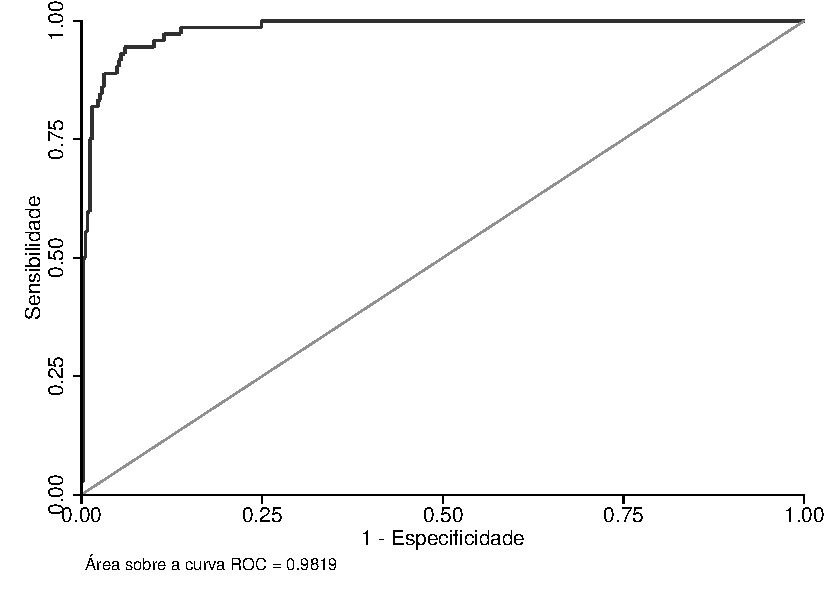
\includegraphics[scale=1]{roc1.pdf}
	\end{center}
	\legend{Fonte: elaboração própria.}
\end{figure}